\documentclass[border=10pt]{standalone}
\usepackage[utf8]{inputenc}
\usepackage{tikz}
\usetikzlibrary{mindmap,shadows}
\usepackage[hidelinks,pdfencoding=auto]{hyperref}
% Information boxes

%***********COMMAND FOR THE INFONBOX*****************
%currently it is not use
\newcommand*{\info}[4][16.3]{%
  \node [ annotation, #3, scale=0.65, text width = #1em,
          inner sep = 2mm ] at (#2) {%
  \list{$\bullet$}{\topsep=0pt\itemsep=0pt\parsep=0pt
    \parskip=0pt\labelwidth=8pt\leftmargin=8pt
    \itemindent=0pt\labelsep=2pt}%
    #4
  \endlist
  };
}
\begin{document}

\tikzstyle{level 1}=[sibling distance=40mm]
\tikzstyle{level 2}=[sibling distance=40mm]
\tikzstyle{level 3}=[sibling distance=40mm]

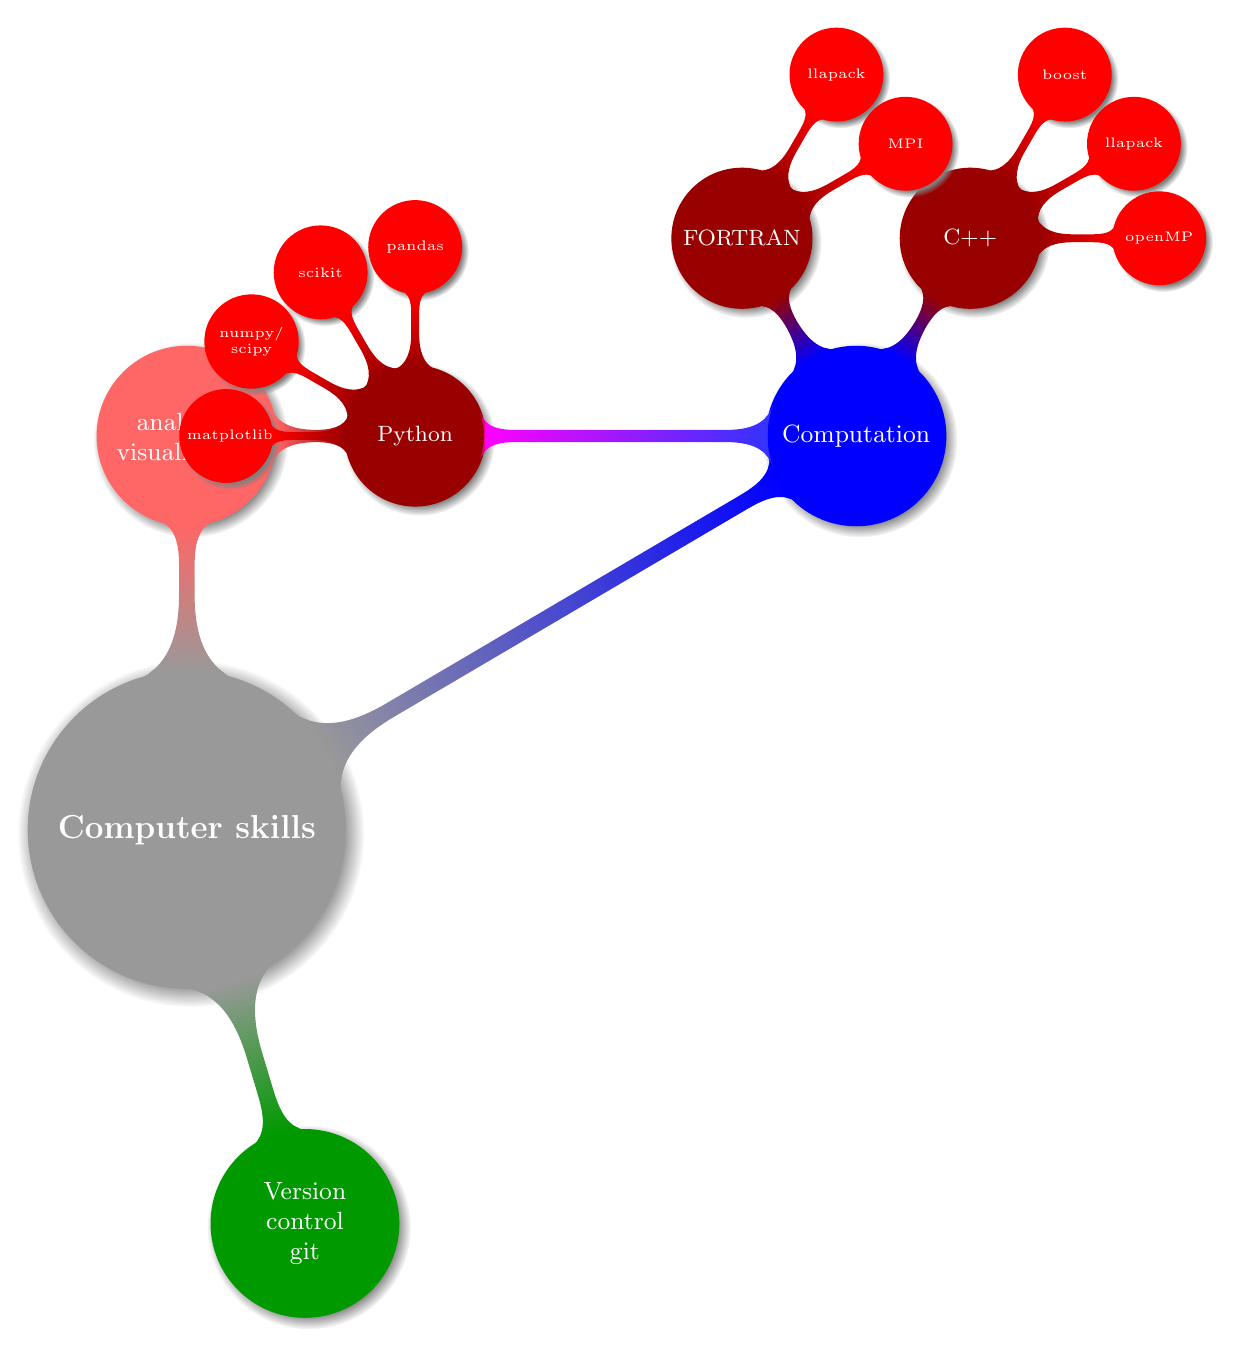
\begin{tikzpicture}[ ]
  \path[mindmap, concept color=black!40, text=white,
        every node/.style={concept,circular drop shadow},
        root/.style    = {concept color=black!40,font=\large\bfseries,text width=10em},
        %level 1 concept/.append style={font=\Large\bfseries, sibling angle=120,text width=7.7em,level distance=15em,inner sep=0pt},
        %level 2 concept/.append style={font=\bfseries,level distance=9em},
      ]
  node[root](CS) at (5,5) {Computer skills}[]
    {
      child[concept color=blue!]
      {
        node(com) at (10,10) {Computation}[counterclockwise from=60]
        {  
          child[concept color=red!60!black]
          {
            node(cpp){C++}[clockwise from=60]
            {
              child[concept color=red]{node(boost){boost}}
              child[concept color=red]{node(llapack){llapack}}
              child[concept color=red]{node(openMP){openMP}}
            }
          }
          child[concept color=red!60!black]
          {
            node{FORTRAN}[clockwise from=60]
            {
              child[concept color=red]{node(llapack2){llapack}}
              child[concept color=red]{node(MPI){MPI}}
            }
          }
        }
      } %close large calculations child
      child[concept color=red!60]
      {
        node(AV) at (0,10) {analysis/\\visualization}[clockwise from=]
        {
          child[concept color=red!60!black]
          {
            node(py){Python}[counterclockwise from=90]
            {
              child[concept color=red]{node(pd){pandas}}
              child[concept color=red]{node(scikit){scikit}}              
              child[concept color=red]{node(np){numpy/ \\ scipy}}
              child[concept color=red]{node(plt){matplotlib}}
            }
          }
        }
      }%close analyss visualization child 
      child[concept color=green!60!black]
      {
        node(VC) at (0,0) {Version\\control\\git} [counterclockwise from=0]
      }  %end version control node
    };% end of the computer skills node
     \path (com) to [circle connection bar switch color=from (blue!80) to (magenta)] (py);

\end{tikzpicture}
\end{document}